% Provenance (never printed): see sources/outline_sources.md (Year 3: the heat
% equation, half-space and plate cooling models, heat flow against age,
% continental geotherms, thermal subsidence). Brief: sources/book5/BRIEFS.md,
% ch. 5. Curves from figdata/bachelor-3/plate_cooling.py (models; Seton et al.
% 2020 age grid and ETOPO1, read only) and continental_geotherm.py.
% Exercise and problem values in the Book 5 scratch calculator calc/ch05.py.
\chapter{Thermische modellen van de lithosfeer}\label{ch:b3:lithosphere-thermal-models}

Vaar weg van een middenoceanische rug en de zeebodem wordt dieper: ongeveer
\qty{2.5}{km} bij de as, meer dan \qty{5}{km} onder de oudste
oceaanbodem. Er is niets aan de plaat toegevoegd of ervan afgenomen; ze is alleen
afgekoeld, gekrompen en gezonken. De oceaanbodem is een thermometer van de plaat
eronder, en een warmtestroomsonde die in het sediment wordt gedrukt, meet dezelfde
afkoeling van bovenaf. Dit hoofdstuk lost de afkoeling van een plaat op twee manieren op, als
een halfruimte en als plaat van eindige dikte, vergelijkt beide met de diepte
van de echte oceaanbodem en zijn warmtestroom, en gaat dan over naar de continenten,
waarvan de warmte deels uit hun eigen korst komt.
% ledger: ps77:depth-age

\begin{recall}
De diffusievergelijking voor warmte, $\partial T/\partial t = \kappa\nabla^2T$,
met de warmtegeleidingscoëfficiënt $k$ en de thermische diffusiviteit $\kappa =
k/(\rho c)$, staat in de natuurkundeboeken; Fourierreeksen en de foutfunctie
$\operatorname{erf}x = (2/\sqrt\pi)\int_0^xe^{-u^2}\,\mathrm du$ staan in de
universitaire delen van de wiskundeboeken. De warmtestroom, de radiogene
warmteproductie, de geotherm, de conductieve tijdschaal $L^2/\kappa$, de thermische
grenslaag en de thermische lithosfeer zijn gedefinieerd in Boek~3,
in het hoofdstuk over de warmtehuishouding van de Aarde; isostasie in het
hoofdstuk over isostasie en zwaartekrachtanomalieën; de diepte--ouderdomswet $d = d_r + C\sqrt t$ werd bewezen in
het hoofdstuk over riften, ruggen en passieve randen, waarbij het temperatuurprofiel
werd aangenomen dat dit hoofdstuk afleidt. Het rekmodel van bekkens, de subsidentie
na de rift en de thermische tijdconstante staan in Boek~4, in het
hoofdstuk over sedimentaire bekkens.
\end{recall}

\section{Conductie, advectie en hun verhouding}

Warmte in de lithosfeer beweegt op twee manieren: ze diffundeert langs de
temperatuurgradiënt, en ze wordt meegevoerd door bewegend gesteente, de plaat die een rug verlaat, een
eroderend bergmassief dat omhoog komt, een magma dat opstijgt. Welke van de twee overheerst, hangt af van
één getal.

\begin{definition}[Thermisch Pécletgetal]\label{def:b3:lithosphere-thermal-models:peclet}
Voor gesteente dat met snelheid $u$ over een lengte $L$ beweegt, is het
\emph{thermische Pécletgetal}\index{thermische Pécletgetal} gelijk aan
\[
  \mathrm{Pe} = \frac{uL}{\kappa},
\]
de verhouding van de conductieve tijd $L^2/\kappa$ tot de advectieve tijd $L/u$.
Advectie overheerst waar $\mathrm{Pe} \gg 1$, conductie waar
$\mathrm{Pe} \ll 1$.
\end{definition}

Een plaat die een rug verlaat met \qty{25}{mm/yr} heeft over een afstand van
\qty{95}{km}, $\mathrm{Pe} \approx 94$ met $\kappa = \qty{0.8e-6}{m^2.s^{-1}}$:
warmte wordt door de plaat zijwaarts veel sneller meegevoerd dan dat ze zijwaarts diffundeert.
Elke verticale kolom van de plaat koelt daarom af alsof ze alleen staat, door verticale
conductie naar de koude zeebodem, waarbij haar ouderdom $t$ staat voor de tijd sinds ze
de as verliet. Zo wordt een probleem in twee dimensies er een in diepte en
tijd.

\section{De afkoelende halfruimte}

\begin{definition}[Halfruimte-afkoelingsmodel]\label{def:b3:lithosphere-thermal-models:half-space}
Het \emph{halfruimte-afkoelingsmodel}\index{halfruimte-afkoelingsmodel} van de
oceanische lithosfeer beschouwt elke kolom als een halfruimte $z \ge 0$ met uniforme
diffusiviteit, op de uniforme temperatuur $T_m$ van de mantel op het moment dat ze
de rugas verlaat, waarvan het oppervlak vanaf dat moment op de temperatuur $T_0$ van de
zeebodem wordt gehouden, zonder warmteproductie en zonder onderkant.
\end{definition}

\begin{theorem}[Foutfunctiegeotherm]\label{thm:b3:lithosphere-thermal-models:erf}
In het \omterm{def:b3:lithosphere-thermal-models:half-space}{halfruimte-afkoelingsmodel} is de temperatuur op de diepte $z$ onder de
zeebodem met ouderdom $t$ gelijk aan
\[
  T(z, t) = T_0 + (T_m - T_0)\operatorname{erf}\frac{z}{2\sqrt{\kappa t}} .
\]
Dit is de \emph{foutfunctiegeotherm}\index{foutfunctiegeotherm}.
\end{theorem}

\begin{proof}
Stel $\theta = (T - T_0)/(T_m - T_0)$; die voldoet aan $\partial\theta/\partial t =
\kappa\,\partial^2\theta/\partial z^2$ met $\theta(z, 0) = 1$ voor $z > 0$ en
$\theta(0, t) = 0$ voor $t > 0$. Het probleem heeft geen eigen lengteschaal:
als $\theta(z, t)$ een oplossing is, dan is ook $\theta(\lambda z, \lambda^2t)$ voor elke
$\lambda > 0$, met dezelfde begin- en randwaarden; omdat de oplossing uniek is, hangt
$\theta$ alleen van $z$ en $t$ af via $\eta = z/(2\sqrt{\kappa
t})$. Met $\theta = f(\eta)$, $\partial\eta/\partial t = -\eta/(2t)$ en
$\partial\eta/\partial z = 1/(2\sqrt{\kappa t})$ geldt
\[
  -\frac{\eta}{2t}f'(\eta) = \kappa\,\frac{f''(\eta)}{4\kappa t},
  \qquad\text{dus}\qquad f'' + 2\eta f' = 0 .
\]
Hieruit volgt $f' = Ae^{-\eta^2}$ en $f = A\int_0^\eta e^{-u^2}\,\mathrm du + B$. De
randvoorwaarde aan het oppervlak, bij $\eta = 0$, geeft $B = 0$; de
beginvoorwaarde, die op elke diepte geldt als $t \to 0$, dat wil zeggen als
$\eta \to \infty$, geeft $A\sqrt\pi/2 = 1$. Dus $f = \operatorname{erf}\eta$.
\end{proof}

De temperatuur op een gegeven diepte hangt alleen af van $z/\sqrt t$: een isotherm zinkt
evenredig met de wortel van de ouderdom, en de afgekoelde laag op \qty{40}{Myr} is twee
keer zo dik als op \qty{10}{Myr}. De warmtestroom aan het oppervlak volgt door differentiëren.

\begin{proposition}[Warmtestroom--ouderdomsrelatie]\label{prop:b3:lithosphere-thermal-models:heat-flow}
In het \omterm{def:b3:lithosphere-thermal-models:half-space}{halfruimte-afkoelingsmodel} is de warmtestroom door de zeebodem met ouderdom $t$
gelijk aan
\[
  q(t) = k\,\frac{\partial T}{\partial z}\Big|_{z=0}
  = \frac{k(T_m - T_0)}{\sqrt{\pi\kappa t}} = \frac{C_q}{\sqrt t} .
\]
\end{proposition}

\begin{proof}
$\partial\operatorname{erf}(z/2\sqrt{\kappa t})/\partial z = (2/\sqrt\pi)
e^{-z^2/4\kappa t}/(2\sqrt{\kappa t})$, die bij $z = 0$ gelijk is aan $1/\sqrt{\pi\kappa
t}$.
\end{proof}

Met de waarden van het plaatmodel hieronder ($k = \qty{3.1}{W.m^{-1}.K^{-1}}$,
$T_m - T_0 = \qty{1450}{K}$, $\kappa = \qty{0.8e-6}{m^2.s^{-1}}$), $C_q =
\qty{505}{mW.m^{-2}.Myr^{1/2}}$, dicht bij de waarden van 430 tot
\qty{510}{mW.m^{-2}.Myr^{1/2}} die verschillende studies op de mondiale metingen hebben aangepast;
studies; een recente compilatie geeft de voorkeur aan \num{490}. Gemeten warmtestroom op jonge
oceanische korst onderschat echter sterk de warmte die de korst verlaat:
zeewater dat door de gebarsten korst circuleert, voert een deel van de warmte weg
in hete bronnen, buiten bereik van de sondes. Op oude korst volgen de metingen
$1/\sqrt t$, en schattingen van het warmteverlies van de Aarde vervangen de
metingen op korst jonger dan \qty{66.5}{Myr} door $C_q/\sqrt t$.
% ledger: honda04:gdh1, b2dd10:half-space, dd10b5:hydrothermal

Boek~3 integreert hetzelfde profiel via isostasie over de diepte, om
de diepte--ouderdomswet te verkrijgen, $d = d_r + C\sqrt t$ met $C = 2\rho_m\alpha(T_m -
T_0)\sqrt\kappa/\bigl(\sqrt\pi(\rho_m - \rho_w)\bigr)$ (figuur hieronder). Met
$\rho_m = \qty{3300}{kg.m^{-3}}$, $\rho_w = \qty{1030}{kg.m^{-3}}$ en $\alpha =
\qty{3.1e-5}{K^{-1}}$, $C = \qty{370}{m.Myr^{-1/2}}$, tegenover de
\qty{350}{m.Myr^{-1/2}} gefit op de zeebodems van de Noord-Pacific en de Noord-Atlantische Oceaan
jonger dan \qty{70}{Myr}.
% ledger: ps77:depth-age

\begin{omfigure}
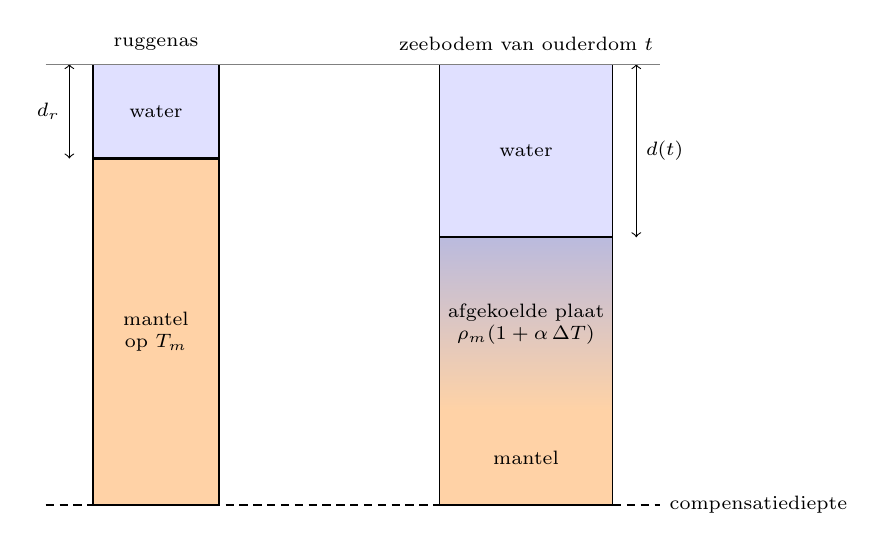
\begin{tikzpicture}[font=\small, x=1cm, y=1cm]
% schematic: two columns of equal mass above the compensation depth
\fill[blue!12] (0,0) rectangle (1.6,-1.2);
\fill[orange!35] (0,-1.2) rectangle (1.6,-5.6);
\fill[blue!12] (4.4,0) rectangle (6.6,-2.2);
\shade[top color=blue!35!gray!40, bottom color=orange!35] (4.4,-2.2) rectangle (6.6,-4.4);
\fill[orange!35] (4.4,-4.4) rectangle (6.6,-5.6);
\draw (0,0) rectangle (1.6,-5.6) (4.4,0) rectangle (6.6,-5.6);
\draw[densely dashed] (-0.6,-5.6) -- (7.2,-5.6) node[right, font=\scriptsize] {compensatiediepte};
\draw[thick] (0,-1.2) -- (1.6,-1.2) (4.4,-2.2) -- (6.6,-2.2);
\node[font=\scriptsize] at (0.8,-0.6) {water};
\node[font=\scriptsize, align=center] at (0.8,-3.4) {mantel\\op $T_m$};
\node[font=\scriptsize] at (5.5,-1.1) {water};
\node[font=\scriptsize, align=center] at (5.5,-3.3) {afgekoelde plaat\\$\rho_m(1 + \alpha\,\Delta T)$};
\node[font=\scriptsize, align=center] at (5.5,-5.0) {mantel};
\draw[<->] (-0.3,0) -- (-0.3,-1.2) node[midway, left, font=\scriptsize] {$d_r$};
\draw[<->] (6.9,0) -- (6.9,-2.2) node[midway, right, font=\scriptsize] {$d(t)$};
\node[above, font=\scriptsize] at (0.8,0.05) {ruggenas};
\node[above, font=\scriptsize] at (5.5,0.05) {zeebodem van ouderdom $t$};
\draw[gray] (-0.6,0) -- (7.2,0);
\end{tikzpicture}

\par\smallskip{\small Isostasie van de afkoelende plaat: de kolom bij de rug
en de kolom van ouderdom $t$ hebben dezelfde massa boven de compensatiediepte. De
afgekoelde, dichtere plaat zinkt en water vult de ruimte
erboven.}\label{fig:b3:lithosphere-thermal-models:columns}
\end{omfigure}

\section{Het plaatmodel}

Oude oceaanbodem wordt niet langer dieper: in de Noord-Pacific en de Noord-Atlantische Oceaan
de diepte wijkt tussen 60 en \qty{80}{Myr} af van $\sqrt t$, en de warmtestroom vlakt af.
De halfruimte blijft voor altijd afkoelen; iets moet de basis van de
plaat warm houden.
% ledger: parsons:plate-model

\begin{definition}[Plaatafkoelingsmodel]\label{def:b3:lithosphere-thermal-models:plate}
Het \emph{plaatafkoelingsmodel}\index{plaatafkoelingsmodel} van de oceanische
lithosfeer beschouwt elke kolom als een laag $0 \le z \le L$ met uniforme
diffusiviteit, op de uniforme temperatuur $T_m$ wanneer ze de rug verlaat, waarvan
het oppervlak op $T_0$ wordt gehouden en waarvan de basis vanaf dat moment op $T_m$ wordt gehouden.
\end{definition}

\begin{theorem}[Temperatuurreeks van het plaatmodel]\label{thm:b3:lithosphere-thermal-models:plate-series}
In het \omterm{def:b3:lithosphere-thermal-models:plate}{plaatafkoelingsmodel}, met $T_0 = 0$,
\[
  T(z, t) = T_m\Bigl[\frac zL + \frac2\pi\sum_{n=1}^\infty\frac1n
  \sin\frac{n\pi z}{L}\,e^{-n^2t/\tau}\Bigr],\qquad
  \tau = \frac{L^2}{\pi^2\kappa} .
\]
Dit is de \emph{temperatuurreeks van het plaatmodel}\index{temperatuurreeks van het plaatmodel}.
\end{theorem}

\begin{proof}
De stationaire toestand, bereikt bij $t \to \infty$, is het lineaire profiel $T_mz/L$.
De afwijking $u = T - T_mz/L$ voldoet aan de diffusievergelijking met $u = 0$ bij
$z = 0$ en $z = L$, en begint als $u(z, 0) = T_m(1 - z/L)$. Door scheiding van de
variabelen, $u = Z(z)\Theta(t)$ levert $Z''/Z = \Theta'/(\kappa\Theta) = -\mu^2$;
de randvoorwaarden laten $Z = \sin(n\pi z/L)$, $\mu = n\pi/L$, en
$\Theta = e^{-n^2\pi^2\kappa t/L^2} = e^{-n^2t/\tau}$. De beginwaarden bepalen de
coëfficiënten $b_n$ van de sinusreeks van $T_m(1 - z/L)$ op $[0, L]$:
\[
  b_n = \frac2L\int_0^LT_m\Bigl(1 - \frac zL\Bigr)\sin\frac{n\pi z}{L}\,\mathrm dz
  = \frac{2T_m}{n\pi},
\]
door partiële integratie. Het optellen van de modi levert de reeks op.
\end{proof}

Elke modus vervalt met zijn eigen tijd, $\tau/n^2$: de hogere harmonischen, de fijne
structuur van de beginsprong, verdwijnen het eerst, en na een tijd van de orde $\tau$
blijft alleen de eerste over. Dezelfde scheiding van variabelen levert de
warmtestroom en, via het isostatische evenwicht van de figuur hierboven, de diepte.

\begin{proposition}[Diepte en warmtestroom van het plaatmodel]\label{prop:b3:lithosphere-thermal-models:plate-depth}
In het \omterm{def:b3:lithosphere-thermal-models:plate}{plaatafkoelingsmodel}, met de dichtheden en de uitzettingscoëfficiënt van de
diepte--ouderdomswet,
\[
  q(t) = \frac{kT_m}{L}\Bigl[1 + 2\sum_{n=1}^\infty e^{-n^2t/\tau}\Bigr],\qquad
  d(t) = d_r + \frac{\rho_m\alpha T_mL}{2(\rho_m - \rho_w)}
  \Bigl[1 - \frac{8}{\pi^2}\sum_{n\ \text{oneven}}\frac{e^{-n^2t/\tau}}{n^2}\Bigr].
\]
Voor $t \to \infty$ nadert de diepte tot $d_r + \rho_m\alpha T_mL/\bigl(2(\rho_m -
\rho_w)\bigr)$ en de warmtestroom naar $kT_m/L$, beide exponentieel, met de
tijdconstante $\tau$.
\end{proposition}

\begin{proof}
Door de reeks in $z = 0$ te differentiëren volgt $\partial T/\partial z = (T_m/L)[1 +
2\sum e^{-n^2t/\tau}]$. Voor de diepte geeft het isostatische evenwicht $(\rho_m -
\rho_w)(d - d_r) = \rho_m\alpha\int_0^L(T_m - T)\,\mathrm dz$. Het lineaire deel
levert $T_mL/2$ op; elke modus levert $-(2T_m/n\pi)e^{-n^2t/\tau}
\int_0^L\sin(n\pi z/L)\,\mathrm dz = -(2T_m/n\pi)(L/n\pi)(1 - \cos n\pi)
e^{-n^2t/\tau}$, wat nul is voor even $n$ en $-(4T_mL/n^2\pi^2)
e^{-n^2t/\tau}$ voor oneven $n$. Het afzonderen van $T_mL/2$ levert de haakjesterm op. Voor $t = 0$
verdwijnt die, omdat $\sum_{n\ \text{oneven}}1/n^2 = \pi^2/8$.
\end{proof}

Het plaatmodel dat de wereldwijde dieptes en warmtestromen het best beschrijft, heeft een plaat
van \qty{95}{km} dik met een basis op \qty{1450}{\celsius}, $\alpha =
\qty{3.1e-5}{K^{-1}}$ en $k = \qty{3.1}{W.m^{-1}.K^{-1}}$, dunner en heter
dan de eerdere \qty{125}{km} en \qty{1350}{\celsius}. Met $\kappa =
\qty{0.8e-6}{m^2.s^{-1}}$ is $\tau = \qty{36.2}{Myr}$; de diepte vlakt af op
$2500 + 3104 = \qty{5604}{m}$ en de warmtestroom op \qty{47}{mW.m^{-2}}. Jonge
oceaanbodem kan de twee modellen niet van elkaar onderscheiden: ze verschillen minder dan een meter
bij \qty{2}{Myr} en met \qty{100}{m} bij \qty{44}{Myr}. Seismologie geeft een vergelijkbaar
antwoord: Rayleighgolven uit de Stille Oceaan worden het best beschreven door afkoelende platen
waarvan de asymptotische dikte van 85 tot \qty{95}{km} is.
% ledger: honda04:gdh1, ps77:depth-age, fischer:lithosphere

\begin{omfigure}
\begin{tikzpicture}
\begin{groupplot}[group style={group size=1 by 2, vertical sep=2.3cm},
  omrecord, width=0.86\linewidth, height=0.42\linewidth, xmin=0, xmax=160,
  xlabel={ouderdom van de zeebodem (Myr)}]
\nextgroupplot[omdepth, ylabel={diepte (km)}, ymin=0, ymax=130,
  title={(a) isothermen, elke \qty{200}{\celsius}}, title style={font=\small},
  legend style={font=\scriptsize, at={(0.01,0.03)}, anchor=south west}]
% computed in figdata/bachelor-3/plate_cooling.py; ledger: honda04:gdh1
\addplot[omDef, thick] table[x=t, y=hs200] {figdata/out/bachelor-3-plate_cooling-isotherms.dat};
\addlegendentry{halfruimte}
\addplot[red!70!black, thick, densely dashed] table[x=t, y=pl200] {figdata/out/bachelor-3-plate_cooling-isotherms.dat};
\addlegendentry{plaat, $L = \qty{95}{km}$}
\foreach \lev in {400,600,800,1000,1200,1400} {
  \addplot[omDef, thick, forget plot] table[x=t, y=hs\lev] {figdata/out/bachelor-3-plate_cooling-isotherms.dat};
  \addplot[red!70!black, thick, densely dashed, forget plot] table[x=t, y=pl\lev] {figdata/out/bachelor-3-plate_cooling-isotherms.dat};
}
\draw[gray] (axis cs:0,95) -- (axis cs:160,95);
\node[font=\scriptsize, anchor=north] at (axis cs:68,96) {basis van de plaat};
\node[font=\scriptsize, fill=white, inner sep=1pt] at (axis cs:150,14) {200};
\node[font=\scriptsize, fill=white, inner sep=1pt] at (axis cs:28,38.2) {1000};
\node[font=\scriptsize, fill=white, inner sep=1pt] at (axis cs:22,70.4) {1400};
\nextgroupplot[ylabel={warmtestroom (\unit{mW.m^{-2}})}, ymin=0, ymax=300,
  title={(b) warmtestroom}, title style={font=\small},
  legend style={font=\scriptsize, at={(0.98,0.97)}, anchor=north east}]
\addplot[omDef, thick] table[x=t, y=hs] {figdata/out/bachelor-3-plate_cooling-heat.dat};
\addlegendentry{halfruimte}
\addplot[red!70!black, thick, densely dashed] table[x=t, y=pl] {figdata/out/bachelor-3-plate_cooling-heat.dat};
\addlegendentry{plaat}
\end{groupplot}
\end{tikzpicture}

\par\smallskip{\small De twee afkoelingsmodellen met de parameters van de tekst.
(a) Diepte van de isothermen van \qty{200}{\celsius} (boven) tot
\qty{1400}{\celsius} (onder): die van de halfruimte blijven zakken als
$\sqrt t$, die van de plaat stoppen zodra het profiel lineair wordt. (b) Oppervlaktewarmtestroom:
het plaatmodel vlakt af op \qty{47}{mW.m^{-2}}, die van de halfruimte
daalt als $1/\sqrt t$.}\label{fig:b3:lithosphere-thermal-models:isotherms}
\end{omfigure}

De echte oceaanbodem kan in dezelfde grafiek worden gezet (figuur hieronder). Elke cel van
één graad in breedte en lengte waarvan de ouderdom bekend is, wordt geplaatst op zijn ouderdom en
zijn diepte; de mediaan van elke bin van vijf miljoen jaar stijgt met de ouderdom,
zoals de modellen dat voor de eerste \qty{40}{Myr} aangeven, maar de waargenomen bodem ligt ondieper dan beide modellen,
en naarmate de ouderdom toeneemt steeds meer. Er is niets gecorrigeerd: oude bodem
draagt een dikkere laag sediment, in de oudere Noord-Atlantische Oceaan meer dan een kilometer, die hem belast
en zijn bovenkant doet stijgen, en oude bodem heeft tijd gehad om
zeebergen, vulkanische plateaus en de welvingen van hotspots te verzamelen. De gepubliceerde
aanpassingen verwijderen eerst de sedimentbelasting en de duidelijke welvingen; de diepte--ouderdomswet van Boek~3 en de plaatmodellen hierboven
komen uit zulke gecorrigeerde
dieptes.
% ledger: data:b5-depth-age, ps77:depth-age

\begin{omfigure}
\begin{tikzpicture}
\begin{axis}[omrecord, omdepth, width=0.86\linewidth, height=0.5\linewidth,
  xmin=0, xmax=180, ymin=2, ymax=6.5, xlabel={ouderdom van de zeebodem (Myr)},
  ylabel={diepte (km)},
  legend style={font=\scriptsize, at={(0.5,-0.24)}, anchor=north, cells={anchor=west}},
  legend columns=2]
% computed in figdata/bachelor-3/plate_cooling.py; ledger: data:b5-depth-age, honda04:gdh1
\addplot[only marks, mark=*, mark size=1.3pt, black,
  error bars/.cd, y dir=both, y explicit]
  table[x=t, y expr=\thisrow{med}/1000, y error plus expr=(\thisrow{q3}-\thisrow{med})/1000,
  y error minus expr=(\thisrow{med}-\thisrow{q1})/1000] {figdata/out/bachelor-3-plate_cooling-bins.dat};
\addlegendentry{waargenomen, mediaan en kwartielen}
\addplot[omDef, thick] table[x=t, y expr=\thisrow{hs}/1000] {figdata/out/bachelor-3-plate_cooling-depth.dat};
\addlegendentry{halfruimte}
\addplot[red!70!black, thick, densely dashed] table[x=t, y expr=\thisrow{pl}/1000] {figdata/out/bachelor-3-plate_cooling-depth.dat};
\addlegendentry{plaat, $L = \qty{95}{km}$}
\end{axis}
\end{tikzpicture}

\par\smallskip{\small Diepte van de oceaanbodem tegen zijn ouderdom: de mediaan en de kwartielen
van de dieptes van de cellen van één graad in elke bin van vijf miljoen jaar
(zeebodem dieper dan \qty{1000}{m}, ouderdommen uit een wereldwijd ouderdomsraster, dieptes uit een wereldwijd reliëfmodel,
geen correctie voor sediment, zeebergen of welvingen),
met de twee afkoelingsmodellen van de tekst.}\label{fig:b3:lithosphere-thermal-models:depth-age}
\end{omfigure}

\begin{definition}[Thermische subsidentie]\label{def:b3:lithosphere-thermal-models:thermal-subsidence}
\emph{Thermische subsidentie}\index{thermische subsidentie} is het dalen van het
oppervlak van de lithosfeer als die afkoelt en krimpt naar thermisch evenwicht,
waarbij de ruimte erboven wordt gevuld door water of sediment; isostasie
zet de door een kolom afgegeven warmte om in haar daling.
\end{definition}

De oceaanbodem is het zuivere geval. Een uitgerekt continentaal bekken is een ander: een
lithosfeer die met een factor $\beta$ is uitgedund, brengt heet asthenosfeer omhoog, en de
post-rift-subsidentie uit Boek~4 is dezelfde plaatafkoeling, startend vanuit een ander
profiel, met dezelfde modi en dezelfde vervaltijden $\tau/n^2$.
Alleen de eerste modus houden is daarom een goede benadering zodra de hogere modi zijn uitgedoofd,
en een slechte ervoor: voor de oceaanbodem van het plaatmodel hierboven geeft de eerste term alleen
de diepte tot binnen twee meter na
\qty{20}{Myr}, maar is hij op \qty{5}{Myr} \qty{84}{m} te diep.

\section{Continentale geotermen}

Continentale korst maakt warmte: graniet bevat uranium, thorium en kalium in
concentraties waardoor de in de bovenste korst geproduceerde warmte een groot deel vormt van
de warmtestroom aan het oppervlak. Hoe de productie met de diepte verdeeld is,
bepaalt de temperatuur op diepte.

\begin{definition}[Diepteschaal van de warmteproductie; gereduceerde warmtestroom]\label{def:b3:lithosphere-thermal-models:reduced}
Wanneer de radiogene warmteproductie van de korst met de diepte afneemt als
$A(z) = A_0e^{-z/h_r}$, is $h_r$ de \emph{diepteschaal van de
warmteproductie}\index{diepteschaal van de warmteproductie}. De \emph{gereduceerde
warmtestroom}\index{gereduceerde warmtestroom} $q_m$ van een provincie is de warmtestroom die
aan het oppervlak zou overblijven als de korst geen warmte zou produceren: de warmtestroom
van onder de radiogene laag.
\end{definition}

\begin{proposition}[Exponentiële warmteproductie]\label{prop:b3:lithosphere-thermal-models:exponential}
In stationaire geleiding met uniforme geleidbaarheid $k$, oppervlaktetemperatuur $0$,
warmteproductie $A_0e^{-z/h_r}$ en warmtestroom $q_m$ vanuit grote diepte, is de
warmtestroom aan het oppervlak
\[
  q_0 = q_m + A_0h_r,
\]
en de geoterm is
\[
  T(z) = \frac{q_mz}{k} + \frac{A_0h_r^2}{k}\bigl(1 - e^{-z/h_r}\bigr).
\]
Als de plutons van een provincie dezelfde $h_r$ en dezelfde $q_m$ delen, liggen hun
warmtestromen aan het oppervlak en hun warmteproducties aan het oppervlak op de rechte lijn
$q_0 = q_m + h_rA_0$.
\end{proposition}

\begin{proof}
In stationaire toestand neemt de opwaartse warmtestroom $q(z) = k\,\mathrm dT/\mathrm dz$ naar boven af
met de geproduceerde warmte: $\mathrm dq/\mathrm dz = -A(z)$. Met $q \to q_m$
op diepte, $q(z) = q_m + A_0h_re^{-z/h_r}$, dus $q_0 = q_m + A_0h_r$. Integreren van
$\mathrm dT/\mathrm dz = q(z)/k$ vanaf $T(0) = 0$ geeft de geoterm. De laatste
bewering is de eerste, gelezen voor elke pluton afzonderlijk.
\end{proof}

De lijn is waargenomen: in verschillende provincies liggen de warmtestromen en de warmteproducties
aan het oppervlak van plutons op rechte lijnen, met diepteschalen van 7.5 tot
\qty{10}{km} en een \omterm{def:b3:lithosphere-thermal-models:reduced}{gereduceerde warmtestroom} van \qty{0.8}{HFU} (ongeveer
\qty{33.5}{mW.m^{-2}}) ten oosten van de Rocky Mountains. De exponentiële vorm is niet
de enige die een lijn geeft, maar hij houdt de lijn intact bij erosie: het verwijderen van een plak met dikte $e$ van bovenaf vermenigvuldigt
$A_0$ en het radiogene deel van $q_0$ met dezelfde factor $e^{-e/h_r}$.
% ledger: b2roy:provinces

Onderstaande figuur toont geotermen voor oppervlaktewarmtestromen van 40, 60 en
\qty{80}{mW.m^{-2}}, de eerste typisch voor cratons en de laatste voor achterboogregio's, met
$k = \qty{2.5}{W.m^{-1}.K^{-1}}$, $h_r = \qty{10}{km}$ en een korstaandeel
$A_0h_r = 0.4\,q_0$. De isotherm van \qty{1300}{\celsius}, genomen als basis van de
thermische lithosfeer, ligt op 129, 84 en \qty{61}{km}.
Seismologie vindt cratonisch mantelgesteente snel tot ongeveer \qty{250}{km}, en de
lithosfeer van achterboogregio's 50 tot \qty{60}{km} dik: de koude, dikke wortels van cratons
hebben een kleinere \omterm{def:b3:lithosphere-thermal-models:reduced}{gereduceerde warmtestroom} nodig dan dit eenvoudige model hen geeft, en hun
geleidbaarheid verandert met de temperatuur, maar de orde van het contrast klopt.
% ledger: hyndman:backarc, fischer:lithosphere, delaney86:properties

\begin{omfigure}
\begin{tikzpicture}
\begin{axis}[omrecord, omdepth, width=0.62\linewidth, height=0.6\linewidth,
  xmin=0, xmax=1600, ymin=0, ymax=200, xlabel={temperatuur (\unit{\celsius})},
  ylabel={diepte (km)},
  legend style={font=\scriptsize, at={(0.02,0.03)}, anchor=south west, cells={anchor=west}}]
% computed in figdata/bachelor-3/continental_geotherm.py
\addplot[black, thick] table[x=T40, y=z] {figdata/out/bachelor-3-continental_geotherm-geotherms.dat};
\addlegendentry{$q_0 = \qty{40}{mW.m^{-2}}$}
\addplot[omDef, thick, densely dashed] table[x=T60, y=z] {figdata/out/bachelor-3-continental_geotherm-geotherms.dat};
\addlegendentry{$q_0 = \qty{60}{mW.m^{-2}}$}
\addplot[red!70!black, thick, dashdotted] table[x=T80, y=z] {figdata/out/bachelor-3-continental_geotherm-geotherms.dat};
\addlegendentry{$q_0 = \qty{80}{mW.m^{-2}}$}
\draw[gray, densely dotted] (axis cs:1300,0) -- (axis cs:1300,200);
\node[font=\scriptsize, rotate=90, anchor=south] at (axis cs:1300,160) {\qty{1300}{\celsius}};
\end{axis}
\end{tikzpicture}

\par\smallskip{\small Stationaire continentale geotermen met exponentieel afnemende
warmteproductie ($h_r = \qty{10}{km}$, $A_0h_r = 0.4\,q_0$, $k =
\qty{2.5}{W.m^{-1}.K^{-1}}$) voor drie oppervlaktewarmtestromen. De kromming nabij
het oppervlak komt van de eigen warmte van de korst; onder enkele diepteschalen is elke
geoterm een rechte lijn met helling $q_m/k$.}\label{fig:b3:lithosphere-thermal-models:geotherms}
\end{omfigure}

\begin{inthefield}[Warmtestroom op zee meten]
\begin{minipage}[t]{0.55\linewidth}\vspace{0pt}
Een marien warmtestroomsensor is een lange stalen lans met een zwaar gewicht bovenop en
een slanke buis met temperatuursensoren langs zijn zijde. Vanaf het achterschip van een
onderzoeksschip wordt hij aan de lierkabel naar de zeebodem gelaten en laat hij zich
met sensoren en al in het zachte sediment vallen. Hij blijft enkele minuten stil
terwijl de wrijvingswarmte van de indringing wegebt en de sensoren zich instellen
op de temperatuur van het slib eromheen; hun metingen, op meters afstand van elkaar, geven
de temperatuurgradiënt. Vervolgens wordt een korte warmtepuls door de buis gestuurd,
en de snelheid waarmee die afneemt geeft de geleidbaarheid van het omringende sediment
; het product van beide is de warmtestroom. De lans wordt eruit getrokken en
weer neergezet, een paar honderd meter verderop langs de lijn, zonder
terug aan dek te komen.
\end{minipage}\hfill
\begin{minipage}[t]{0.42\linewidth}\vspace{0pt}
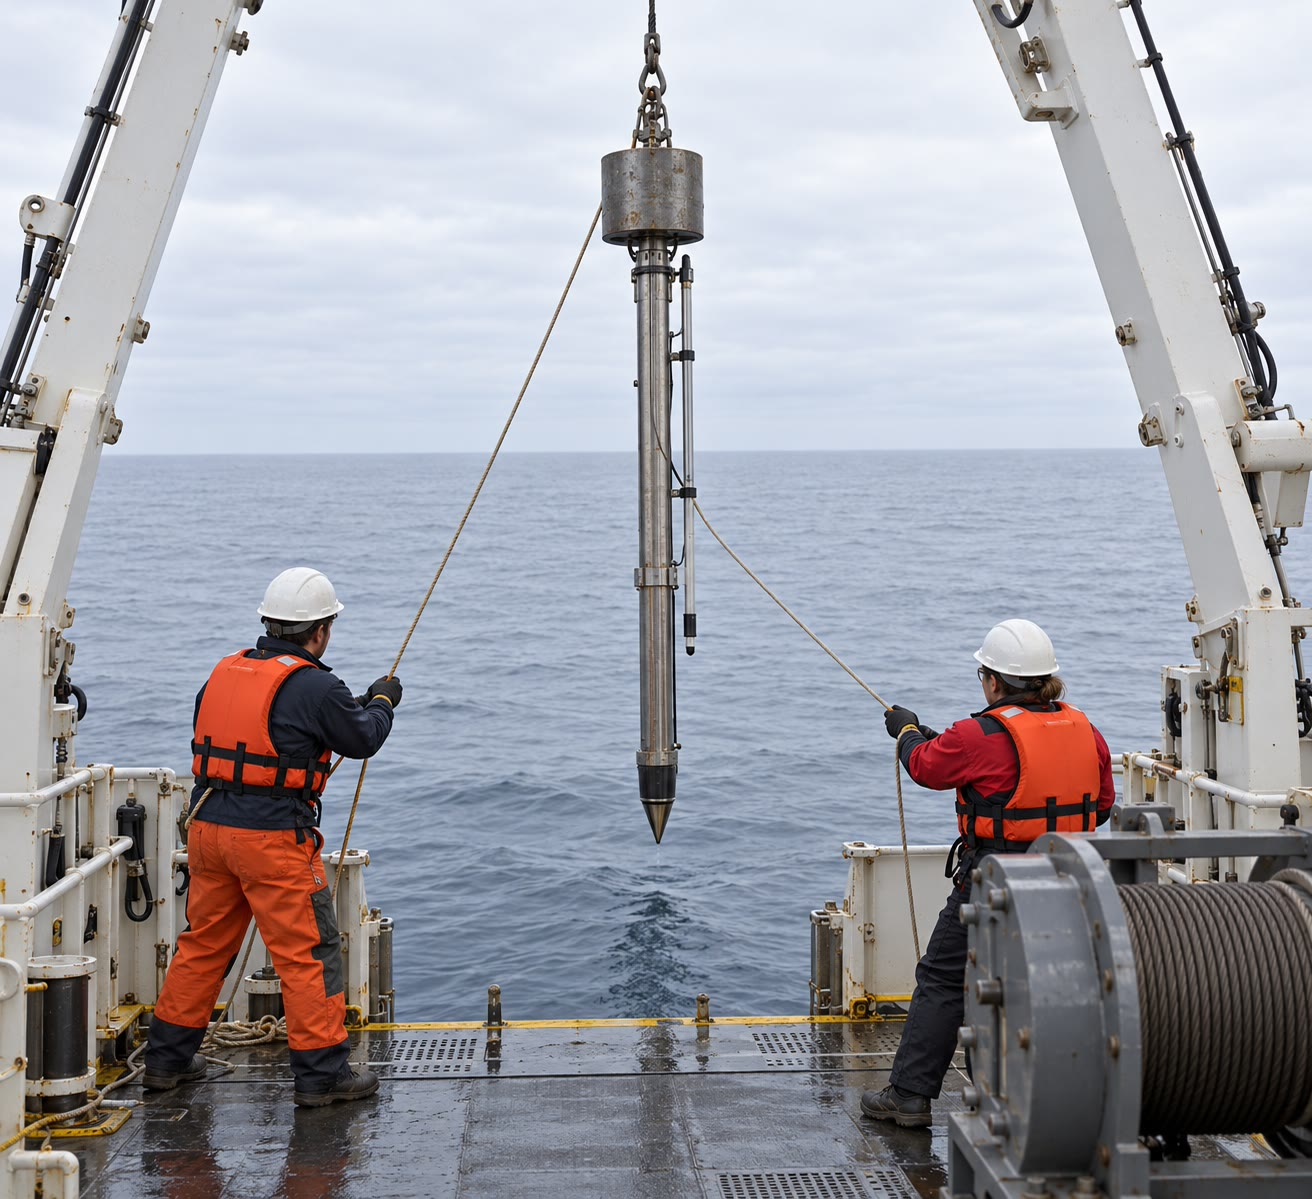
\includegraphics[width=\linewidth]{images/book5/ai/b3-heatflow-probe.jpg}

{\scriptsize Een warmtestroomlans die op het punt staat te worden neergelaten vanaf het
achterschip van een onderzoeksschip (Door AI gegenereerde illustratie.)}
\end{minipage}
\end{inthefield}

\section{Oefeningen}

\begin{exercise}[$\star$]\label{exo:b3:lithosphere-thermal-models:1}
Met $\kappa = \qty{e-6}{m^2.s^{-1}}$ bereken de conductieve tijd $L^2/\kappa$
voor $L = 1$, 10 en \qty{100}{km}, in miljoen jaar.
\end{exercise}

\begin{exercise}[$\star$]\label{exo:b3:lithosphere-thermal-models:2}
Een gebergte wordt geërodeerd met \qty{1}{mm/yr}, en gesteente stijgt door de bovenste
\qty{30}{km} van de korst om het te vervangen. Met $\kappa = \qty{e-6}{m^2.s^{-1}}$,
bereken het Pécletgetal. Kan de geotherm van het gebergte worden berekend
met uitsluitend geleiding?
\end{exercise}

\begin{exercise}[$\star$]\label{exo:b3:lithosphere-thermal-models:3}
In het halfruimtemodel ($T_0 = 0$, $T_m = \qty{1450}{\celsius}$, $\kappa =
\qty{0.8e-6}{m^2.s^{-1}}$), bereken de temperatuur \qty{10}{km} onder de
zeebodem van \qty{5}{Myr} oud (\qty{1}{Myr} $= \qty{3.156e13}{s}$; $\operatorname{erf}
0.445 = 0.471$).
\end{exercise}

\begin{exercise}[$\star$]\label{exo:b3:lithosphere-thermal-models:4}
Met $C_q = \qty{490}{mW.m^{-2}.Myr^{1/2}}$ bereken de warmtestroom door
de zeebodem van 1, 25 en \qty{100}{Myr} oud. Welke van de drie zou een sonde
waarschijnlijk het sterkst onderschatten?
\end{exercise}

\begin{exercise}[$\star\star$]\label{exo:b3:lithosphere-thermal-models:5}
In het halfruimtemodel bereikt de temperatuur \qty{90}{\percent} van $T_m$
waar $\operatorname{erf}\eta = 0.9$, $\eta = 1.163$. Met $\kappa =
\qty{0.8e-6}{m^2.s^{-1}}$ bereken die diepte bij 10, 40 en \qty{100}{Myr}.
\end{exercise}

\begin{exercise}[$\star\star$]\label{exo:b3:lithosphere-thermal-models:6}
Met de waarden uit de tekst levert het halfruimtemodel $C =
\qty{370.5}{m.Myr^{-1/2}}$. Houd alle andere waarden gelijk; welke thermische
uitzettingscoëfficiënt geeft de aangepaste \qty{350}{m.Myr^{-1/2}}? Welke andere
parameter zou in plaats daarvan veranderd kunnen worden?
\end{exercise}

\begin{exercise}[$\star\star$]\label{exo:b3:lithosphere-thermal-models:7}
Bereken de asymptotische warmtestroom $kT_m/L$ van het plaatmodel voor $L =
\qty{95}{km}$, $T_m = \qty{1450}{\celsius}$, en voor $L = \qty{125}{km}$,
$T_m = \qty{1350}{\celsius}$, met $k = \qty{3.1}{W.m^{-1}.K^{-1}}$ in beide gevallen.
Welke ligt dichter bij de warmtestroom van oude oceaanbodem, berekend uit $C_q/\sqrt t$
bij \qty{150}{Myr} met $C_q = \qty{490}{mW.m^{-2}.Myr^{1/2}}$?
\end{exercise}

\begin{exercise}[$\star\star$]\label{exo:b3:lithosphere-thermal-models:8}
Een geologische provincie heeft $q_0 = \qty{60}{mW.m^{-2}}$, $h_r = \qty{10}{km}$ en $A_0h_r =
0.4\,q_0$. Bereken $A_0$, $q_m$ en de temperatuur bij de Moho, \qty{35}{km}
diep, met $k = \qty{2.5}{W.m^{-1}.K^{-1}}$.
\end{exercise}

\begin{exercise}[$\star\star$]\label{exo:b3:lithosphere-thermal-models:9}
Twee granietplutons van één provincie geven $q_0 = \qty{66}{mW.m^{-2}}$ met $A_0
= \qty{3.0}{\micro W.m^{-3}}$, en $q_0 = \qty{48}{mW.m^{-2}}$ met $A_0 =
\qty{1.2}{\micro W.m^{-3}}$. Neem aan dat ze op de lijn van
\cref{prop:b3:lithosphere-thermal-models:exponential} liggen; bereken $h_r$ en $q_m$.
\end{exercise}

\begin{exercise}[$\star\star\star$]\label{exo:b3:lithosphere-thermal-models:10}
(a) Toon aan dat de warmte die per oppervlakte-eenheid tussen ouderdom 0 en $t$
via de zeebodem verloren gaat, bedraagt $Q(t) = 2k(T_m - T_0)\sqrt{t/(\pi\kappa)}$ in het
halfruimtemodel. (b) Toon aan dat de subsidentie gelijk is aan $d - d_r = \alpha Q/\bigl(c(\rho_m -
\rho_w)\bigr)$, waarin $c = k/(\rho_m\kappa)$ de soortelijke warmte is. (c) Controleer het
numeriek bij \qty{40}{Myr} met de waarden uit de tekst.
\end{exercise}

\begin{exercise}[$\star\star\star$]\label{exo:b3:lithosphere-thermal-models:11}
In het plaatmodel uit de tekst ($\tau = \qty{36.2}{Myr}$, $\rho_m\alpha T_mL/
\bigl(2(\rho_m - \rho_w)\bigr) = \qty{3104}{m}$), de diepte berekend met de
eerste Fourierterm alleen overschrijdt de volledige reeks vooral door de term met $n = 3$.
Bereken de grootte van die term bij 1, 10 en \qty{20}{Myr}, en de ouderdom waarna
de eerste term alleen binnen \qty{10}{m} van de reeks ligt.
\end{exercise}

\begin{exercise}[$\star\star\star$]\label{exo:b3:lithosphere-thermal-models:12}
(a) Toon aan dat in de geotherm van \cref{prop:b3:lithosphere-thermal-models:exponential},
$T(z) \approx q_mz/k + A_0h_r^2/k$ voor $z \gg h_r$. (b) Leid de diepte af van de isotherm van
\qty{1300}{\celsius} voor $q_0 = \qty{40}{mW.m^{-2}}$, met de waarden van
oefening 8. (c) Met hoeveel moet $q_m$ dalen opdat die diepte
\qty{250}{km} bereikt, de diepte van de snelle wortels van cratons?
\end{exercise}

\section{Probleem: Veertig miljoen jaar weg van de rug}

\begin{problem}[{Weekendprobleem --- het halfruimtemodel en het plaatmodel, de diepte van
een verzonnen oceaan, en de dikte van de plaat ervan}]
\label{pb:b3:lithosphere-thermal-models:1}
% values: calc/ch05.py; plate_cooling.py; honda04:gdh1, ps77:depth-age, data:b5-depth-age
Neem $T_0 = 0$, $T_m = \qty{1450}{\celsius}$, $\kappa =
\qty{0.8e-6}{m^2.s^{-1}}$, $k = \qty{3.1}{W.m^{-1}.K^{-1}}$, $\alpha =
\qty{3.1e-5}{K^{-1}}$, $\rho_m = \qty{3300}{kg.m^{-3}}$, $\rho_w =
\qty{1030}{kg.m^{-3}}$, een rug die \qty{2500}{m} diep ligt, en \qty{1}{Myr} $=
\qty{3.156e13}{s}$.

\medskip\noindent\textbf{Deel I --- Het halfruimtemodel.}
\begin{enumerate}
  \item Bereken $\sqrt{\kappa t}$ bij 10 en \qty{40}{Myr}.
  \item Bereken de temperatuur \qty{20}{km} onder de zeebodem op beide ouderdommen
        ($\operatorname{erf}0.6294 = 0.6266$, $\operatorname{erf}0.3147 =
        0.3437$).
  \item De isotherm van \qty{1000}{\celsius} ligt waar $\operatorname{erf}\eta =
        0.6897$, $\eta = 0.7174$. Bereken de diepte ervan op beide ouderdommen, en de ouderdom
        waarop ze \qty{60}{km} bereikt.
  \item Bereken de warmtestroom op beide ouderdommen, en $C_q$.
  \item Een rug spreidt zich met \qty{25}{mm/yr} aan elke kant. Bereken het Pécletgetal
        van de plaat over \qty{95}{km}. Waarom mag elke kolom alleen
        worden afgekoeld?
  \item Bereken de conductieve tijd over \qty{95}{km}. Wat zegt die over
        een halfruimtemodel van een zeebodem van \qty{150}{Myr} oud?
\end{enumerate}

\medskip\noindent\textbf{Deel II --- Subsidentie.}
\begin{enumerate}[resume]
  \item Herhaal het isostatisch evenwicht dat het temperatuurtekort van een
        kolom omzet in subsidentie, en waarom de integraal tot oneindig mag worden genomen
        in de halfruimte.
  \item Bereken $C$ van de diepte--ouderdomswet, en de diepten op 10 en
        \qty{40}{Myr}.
  \item De mediane diepte van de echte oceaanbodem tussen 40 en \qty{45}{Myr}
        is \qty{4475}{m}, ongecorrigeerd. Vergelijk met het model op
        \qty{42.5}{Myr}, en noem op wat de mediaan bevat dat het model
        weglaat.
  \item Hoeveel zou $C$ veranderen als $T_m$ \qty{1350}{\celsius} zou zijn?
        Vergelijk met de gefitte \qty{350}{m.Myr^{-1/2}}.
  \item Waarom vallen gemeten warmtestromen op jonge bodem lager uit dan $C_q/\sqrt t$?
\end{enumerate}

\medskip\noindent\textbf{Deel III --- De plaat.} Neem $L = \qty{95}{km}$.
\begin{enumerate}[resume]
  \item Bereken $\tau$ en de amplitude $\rho_m\alpha T_mL/\bigl(2(\rho_m -
        \rho_w)\bigr)$.
  \item Bereken de diepte op \qty{40}{Myr} met de termen $n = 1$, 3 en 5.
  \item Hoeveel verschilt de eerste term alleen daarvan, en waarom zo
        weinig?
  \item Bereken het verschil tussen de halfruimte en de plaat op 40 en
        \qty{50}{Myr}, en schat door lineaire interpolatie de ouderdom waarop
        het \qty{100}{m} bereikt.
  \item Bereken de warmtestroom van de plaat op \qty{40}{Myr}, met de termen
        $n = 1$ tot 3, en vergelijk met de halfruimte.
  \item Geef de asymptotische diepte en warmtestroom.
\end{enumerate}

\medskip\noindent\textbf{Deel IV --- Een verzonnen oceaan.} In een verzonnen oceaan
waarvan de rug \qty{2500}{m} diep is, is de bodem, na correctie voor sediment
en weg van zeebergen en drempels, is \qty{5700}{m} diep op \qty{120}{Myr} en
\qty{4800}{m} op \qty{40}{Myr}. De $L$ van de plaat is onbekend; alle andere
waarden zijn als hierboven.
\begin{enumerate}[resume]
  \item Houd alleen de eerste Fourierterm aan en schrijf de diepte op
        \qty{120}{Myr} als functie van $L$, waarbij $\tau$ zelf van
        $L$ afhangt.
  \item Los het op naar $L$ door iteratie, startend bij $L = \qty{100}{km}$:
        bereken $\tau$, dan de $L$ die \qty{5700}{m} geeft bij die
        $\tau$, en herhaal.
  \item Bereken met de gevonden $L$ de diepte op \qty{40}{Myr} en vergelijk
        met de halfruimte en met de gemeten \qty{4800}{m}.
  \item Bereken $\tau$ voor die $L$ en de asymptotische diepte van deze oceaan.
  \item Na welke ouderdom ligt de bodem binnen \qty{100}{m} van zijn
        asymptotische diepte?
  \item Geef de dikte $L$ van de plaat die bij de oude bodem van de
        verzonnen oceaan past.
\end{enumerate}
\end{problem}
